\documentclass[a4paper]{article}
\usepackage[utf8]{inputenc}
\usepackage[ngerman]{babel}
\usepackage{listings}
\usepackage{float}
\usepackage{graphicx}
\usepackage{color}
\usepackage{listings}
\usepackage[dvipsnames]{xcolor}
\usepackage{tabularx}
\usepackage{geometry}
\usepackage{color,graphicx,overpic}
\usepackage{amsmath,amsthm,amsfonts,amssymb}
\usepackage{tabularx}
\usepackage{listings}
\usepackage[many]{tcolorbox}
\usepackage{multicol}

\newtheorem{definition}{Definition}
\newtheorem{proposition}{Proposition}
\newtheorem{beweis}{Beweis}

\pdfinfo{
    /Title (Automaten, Sprachen \& Komplexität - Übung)
    /Creator (TeX)
    /Producer (pdfTeX 1.40.0)
    /Author (Robert Jeutter)
    /Subject ()
}

% Don't print section numbers
\setcounter{secnumdepth}{0}

%My Environments
\newtheorem{example}[section]{Example}


\newtcolorbox{myboxii}[1][]{
  breakable,
  freelance,
  title=#1,
  colback=white,
  colbacktitle=white,
  coltitle=black,
  fonttitle=\bfseries,
  bottomrule=0pt,
  boxrule=0pt,
  colframe=white,
  overlay unbroken and first={
  \draw[red!75!black,line width=3pt]
    ([xshift=5pt]frame.north west) -- 
    (frame.north west) -- 
    (frame.south west);
  \draw[red!75!black,line width=3pt]
    ([xshift=-5pt]frame.north east) -- 
    (frame.north east) -- 
    (frame.south east);
  },
  overlay unbroken app={
  \draw[red!75!black,line width=3pt,line cap=rect]
    (frame.south west) -- 
    ([xshift=5pt]frame.south west);
  \draw[red!75!black,line width=3pt,line cap=rect]
    (frame.south east) -- 
    ([xshift=-5pt]frame.south east);
  },
  overlay middle and last={
  \draw[red!75!black,line width=3pt]
    (frame.north west) -- 
    (frame.south west);
  \draw[red!75!black,line width=3pt]
    (frame.north east) -- 
    (frame.south east);
  },
  overlay last app={
  \draw[red!75!black,line width=3pt,line cap=rect]
    (frame.south west) --
    ([xshift=5pt]frame.south west);
  \draw[red!75!black,line width=3pt,line cap=rect]
    (frame.south east) --
    ([xshift=-5pt]frame.south east);
  },
}

\begin{document}
\begin{myboxii}[Disclaimer]
    Die Übungen die hier gezeigt werden stammen aus der Vorlesung \textit{Algorithmen, Sprachen und Komplexität}! Für die Richtigkeit der Lösungen wird keine Gewähr gegeben.
\end{myboxii}


%%%%%%%%%%%%%%%%%%%%%%%%%%%%%%%%%%%%%%%%%%%%%%%%%%%%%%%%%%%%%%%%%%%%%%%%%%%%%%%%%%%%%%%%%%%%%%%%%%%%%%%%%%%%%%%%%%%%
\section{Übung 00}
%##########################################
\subsection{Aufgabe 1}
\textit{Das Schubfachprinzip besagt: Wenn $n$ Objekte auf $m$ Schubladen verteilt werden mit $n > m > 0$, dann gibt es eine Schublade, die mindestens zwei Objekte enthält.}
\textit{Zeigen Sie, dass es mindestens zwei Personen in Deutschland mit gleich vielen Haaren gibt.}

\textit{(b) Beweisen Sie das verschärfte Schubfachprinzip: Verteilt man n Objekte auf m Schubladen mit $n > m > 0$, dann gibt es eine Schublade, die mindestens $\lceil \frac{n}{m}\rceil$ Objekte enthält}

%##########################################
\subsection{Aufgabe 2}
\textit{Zeigen Sie per vollständiger Induktion über $n\geq 0$, dass es in jedem Binärbaum mit mindestens $2^n$ Blättern einen Pfad der Länge mindestens $n$ von der Wurzel zu einem Blatt gibt.}

%##########################################
\subsection{Aufgabe 3}
\textit{Eine Menge A heißt gleichmächtig zu einer Menge B, wenn es eine Bijektion von A nach B gibt. Zeigen Sie:}

\textit{(a) Die Menge der natürlichen Zahlen $\mathbb{N}$ ist nicht gleichmächtig zur Menge der reellen Zahlen $\mathbb{R}$.}

\textit{(b) Keine Menge ist gleichmächtig zu ihrer Potenzmenge. (Satz von Cantor)}

\newpage
%%%%%%%%%%%%%%%%%%%%%%%%%%%%%%%%%%%%%%%%%%%%%%%%%%%%%%%%%%%%%%%%%%%%%%%%%%%%%%%%%%%%%%%%%%%%%%%%%%%%%%%%%%%%%%%%%%%%
\section{Übung 01}
%##########################################
\subsection{Aufgabe 1}
\textit{Es sind die DFAs $M_1$ und $M_2$ und die NFAs $M_3$ und $M_4$ (von links nach rechts) gegeben.}
\begin{center}
    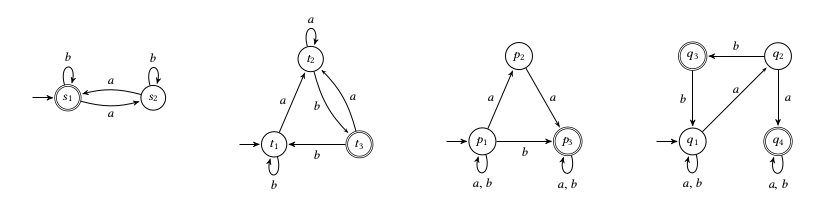
\includegraphics[width=1\linewidth]{Assets/ASK_uebung/u01-01.png}
\end{center}
\textit{Bearbeiten Sie die folgenden Teilaufgaben für alle $i\in \{1, 2, 3, 4\}$.}

\textit{(a) Geben Sie jeweils zwei Wörter an, die von $M_i$ akzeptiert bzw. nicht akzeptiert werden.}

\textit{(b) Geben Sie analog zu Aufgabe 2 eine kurze aber präzise Beschreibung der Sprache $L(M_i)$ an.}


%##########################################
\subsection{Aufgabe 2}
\textit{Betrachten Sie die nachfolgenden Sprachen über dem Alphabet $\sum = \{a, b\}$.
    \begin{itemize}
        \item $L_1 = \{w \in\sum^* \vert \text{w enthält die Zeichenfolge baba}\}$
        \item $L_2 = \sum^* \backslash \{aa, ab, aab\}$
        \item $L_3 = \{w \in\sum^* \vert \text{es existiert } k \geq 1 \text{, so dass w mit } a(ab)^k \text{ beginnt}\}$
        \item $L_4 = \{w\in\sum^* \vert \text{w endet auf aab}\}$
    \end{itemize}
    Geben Sie für alle $i\in\{1, 2, 3, 4\}$ jeweils einen DFA $M_i$ mit $L(M_i)=L_i$ grafisch an. Wählen Sie jeweils zwei Wörter aus $L_i$ und $\sum^*\backslash L_i$ aus und überprüfen Sie, ob $M_i$ auf diesen korrekt arbeitet.}

%##########################################
\subsection{Aufgabe 3}
\textit{Konstruieren Sie mit der Potenzmengenkonstruktion einen DFA, der die gleiche Sprache akzeptiert, wie $M_3$ aus Aufgabe 1.}

%##########################################
\subsection{Aufgabe 4}
\textit{Sei $\sum = \{a, b, c\}$. Unter den folgenden 16 Sprachen über $\sum$ befinden sich acht Paare gleicher Sprachen. Finden Sie heraus, welche Sprachen gleich sind und begründen Sie jeweils in maximal zwei Sätzen, warum die entsprechende Gleichheit gilt.}
\begin{multicols}{2}
    $$L_1 = \{w \in \sum^* \vert \quad\vert w\vert_a = \vert w\vert_b = \vert w\vert_c \}$$
    $$L_2 = \{w \in \sum^* \vert \quad\vert w\vert_a = \vert w\vert_b \}$$
    $$L_3 = \{w \in \sum^* \vert \quad\vert w\vert_a = 0\}$$
    $$L_4 = \{w \in \sum^* \vert \quad\vert w\vert_a = 2\}$$
    $$L_5 = \{w \in \sum^* \vert \quad\vert w\vert_a = 4\}$$
    $$L_6 = \{b, c\}^*\{a\}\{b, c\}^* \{a\}\{b, c\}^*$$
    $$L_7 = \{a\}\{ba\}^*\{b\}$$
    $$L_8 = \{a^n b^n \vert n \in \mathbb{N}\}$$
    $$L_9 = L_2 \cap \{a\}^*\{b\}^*$$
    $$L_{10} = L_2 \cap \{w \in \sum^* \vert \quad\vert w \vert_b = \vert w\vert_c\}$$
    $$L_{11} = (L_3 L_4 )^2$$
    $$L_{12} = \sum^* \backslash L_3$$
    $$L_{13} = L_2^3$$
    $$L_{14} = \{ab\}^+$$
    $$L_{15} = \{b, c\}^*$$
    $$L_{16} = \sum^* \{a\}\sum^*$$
\end{multicols}

%##########################################
\subsection{Aufgabe 5}
\textit{Sei $\sum=\{a, b\}$. Für $n\in\mathbb{N}$ sei $\sum^{\leq n} = \bigcup_{i\leq n} \sum^i$ die Menge der Wörter in $\sum$ deren Länge höchstens $n$ ist. Zeigen Sie per vollständiger Induktion über $n\in\mathbb{N}$, dass $\vert\sum^{\leq n}\vert = 2^{n+1} - 1$.}

%##########################################
\subsection{Aufgabe 6}
\textit{Gegeben sei die Grammatik $G = (\{S, A, B, C\}, \{a, b, c\}, P, S)$, wobei P genau die folgenden Produktionen enthält:
    \begin{multicols}{3}
        $$S\rightarrow A \vert C$$
        $$A \rightarrow Aa \vert a$$
        $$Bb \rightarrow bb$$
        $$Bc \rightarrow bbc$$
        $$C \rightarrow BCc \vert c.$$
    \end{multicols}
}

\textit{(a) Geben Sie eine Ableitung von bbbccc an.}

\textit{(b) Geben Sie eine möglichst kurze aber präzise Beschreibung von L(G) an. Begründen Sie Ihre Antwort.}

%##########################################
\subsection{Aufgabe 7}
\textit{Konstruieren Sie Grammatiken $G_1, G_2$ und $G_3$ so, dass folgende Sprachen erzeugt werden.}

\textit{(a) $L(G_1)=\sum^*\{a\}\sum^*\cup\sum^*\{b\}\sum^*$ für $\sum=\{a,b,c\}$}

\textit{(b) $L(G_2 ) = \{ww^R \vert w \in \{a, b\}^*: \text{w startet mit einem b}\}$ Hinweis:
Für $w=w_1w_2...w_{n-1}w_n$
sei $w^{R} = w_{n} w_{n-1} ... w_{2} w_{1}$ das umgekehrte Wort.}

\textit{(c) $L(G_3)$ ist die Menge der Polynomgleichungen über den Variablen x, y.
    Hinweis: Ein Polynom über den Variablen x, y ist induktiv wie folgt definiert: $0, 1, x, y$ sind Polynome und falls $f,g$ Polynome sind, so auch $(f+g)$ und $(f*g)$.}

\newpage
%%%%%%%%%%%%%%%%%%%%%%%%%%%%%%%%%%%%%%%%%%%%%%%%%%%%%%%%%%%%%%%%%%%%%%%%%%%%%%%%%%%%%%%%%%%%%%%%%%%%%%%%%%%%%%%%%%%%
\section{Übung 02}
%##########################################
\subsection{Aufgabe 1}
\textit{Geben Sie zu den Sprachen $L_a,L_b$ reguläre Ausdrücke $\alpha,\beta$ so an, dass $L(\alpha) = L_a$ und $L(\beta) = L_b$.}

\textit{(a) $L_a = \{w\in\{a, b, c\}^*\vert\text{ entweder kommen a und b in w vor oder weder a noch b}\}$}

\textit{(b) $L_b = \{w\in\{a, b, c\}^*\vert\text{w enthält nicht das Infix bc}\}$}

%##########################################
\subsection{Aufgabe 2}
\textit{Zeigen Sie, dass die Klasse der regulären Sprachen nicht unter unendlicher Vereinigung abgeschlossen ist.}

%##########################################
\subsection{Aufgabe 3}
\textit{Sei $L\subseteq\sum^*$ eine Sprache. Unter der Verdopplung von L verstehen wir die Sprache $2*L:= \{ww \vert w \in L\}$. Überprüfen Sie, ob die Klasse der regulären Sprachen unter Verdopplung abgeschlossen ist. Beweisen Sie Ihre Behauptung!}

%##########################################
\subsection{Aufgabe 4}
\textit{Sei $\sum$ ein Alphabet (eine endliche Menge). Zeigen Sie, dass $\sum^*$ abzählbar ist.}

%##########################################
\subsection{Aufgabe 5}
\textit{Bearbeiten Sie folgende Teilaufgaben:}

\textit{(a) Beschreiben Sie die Sprache des folgenden Automaten kurz und präzise}
\begin{center}
    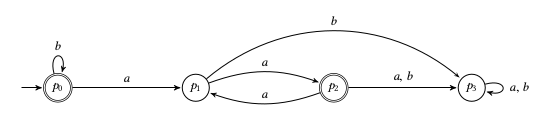
\includegraphics[width=1\linewidth]{Assets/ASK_uebung/u02-01.png}
\end{center}
\textit{(b) Sei $\sum = \{a, b, c\}$. Geben Sie einen DFA an, der die Sprache $L = \{w\in\sum^*\vert |w|_a \leq 1 \text{ und } |w|_b = 0\}$ akzeptiert. Dabei steht für $x\in\sum, w\in\sum^*$ der Ausdruck $|w|_x$ für die Anzahl der x in w.}

%##########################################
\subsection{Aufgabe 6}
\textit{Gegeben seien die folgenden DFAs $M_1$ und $M_2$.}
\begin{center}
    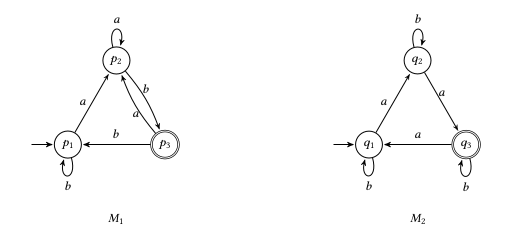
\includegraphics[width=1\linewidth]{Assets/ASK_uebung/u02-02.png}
\end{center}
\textit{Konstruieren Sie folgende Automaten:
    \begin{itemize}
        \item (a) einen DFA $M_\cap$ mit $L(M_\cap) = L(M_1) \cap L(M_2)$,
        \item (b) einen NFA $M_.$ mit $L(M_.) = L(M_1)*L(M_2)$ und
        \item (c) einen NFA $M_* mit L(M_*) = L(M_1)^*$.
    \end{itemize}
}

%##########################################
\subsection{Aufgabe 7}
\textit{Zeigen Sie die folgenden Aussagen:}

\textit{(a) Für jeden NFA $M = (Z , \sum, S, \delta, E)$ existiert ein NFA $M_0 = (Z_0 , \sum, S_0 , \delta_0 , E_0)$ mit $L(M) = L(M_0)$ und $|E_0|=1$.}

\textit{(b) Für jeden NFA $M=(Z,\sum,S,\delta,E)$ existiert ein NFA $M_0=(Z_ 0,\sum,S_0,\delta_0,E_0)$ mit $L(M)=L(M_0)$, $|S_0|=1$ und $|Z_0|=|Z|+1$.}

%##########################################
\subsection{Aufgabe 8}
\textit{Die Spiegelung eines Wortes $w=a_1a_2...a_n\in\sum^*$ sei $w^R := a_na_{n-1}...a_1$ für $a_i\in\sum$ für alle $1\leq i \leq n$. Die Spiegelung einer Sprache $L$ sei $L^R := \{w^R \vert w\in L\}$. Zeigen Sie, dass die Klasse der regulären Sprachen unter Spiegelung abgeschlossen ist.}

\newpage
%%%%%%%%%%%%%%%%%%%%%%%%%%%%%%%%%%%%%%%%%%%%%%%%%%%%%%%%%%%%%%%%%%%%%%%%%%%%%%%%%%%%%%%%%%%%%%%%%%%%%%%%%%%%%%%%%%%%
\section{Übung 03}
%##########################################
\subsection{Aufgabe 1}
\textit{Betrachten Sie die nachfolgenden Sprachen über dem Alphabet $\sum = \{a, b\}$.
    \begin{itemize}
        \item $L_1 = \{w\in\sum^*\vert\text{der vorletzte Buchstabe von w ist ein a}\}$
        \item $L_1 = \sum^*\backslash \{ aa, ab, aab\}$
        \item $L_3 = \{w\in\sum^*\vert\text{ in w kommt ein Buchstabe zweimal direkt hintereinander vor}\}$
        \item $L_4 = \sum^*\backslash L_3$
    \end{itemize}
    Konstruieren Sie für alle $i\in\{1, 2, 3, 4\}$ jeweils einen regulären Ausdruck $r_i$ mit $L(r_i) = L_i$.
}
$$L_1 = (a+b)^* a (a+b)$$

$$L_2 = (b(a+b)^*)+ab(a+b)(a+b)^*+aaa(a+b)^*+aab(a+b)(a+b)^*+a+\lambda$$
\begin{center}
    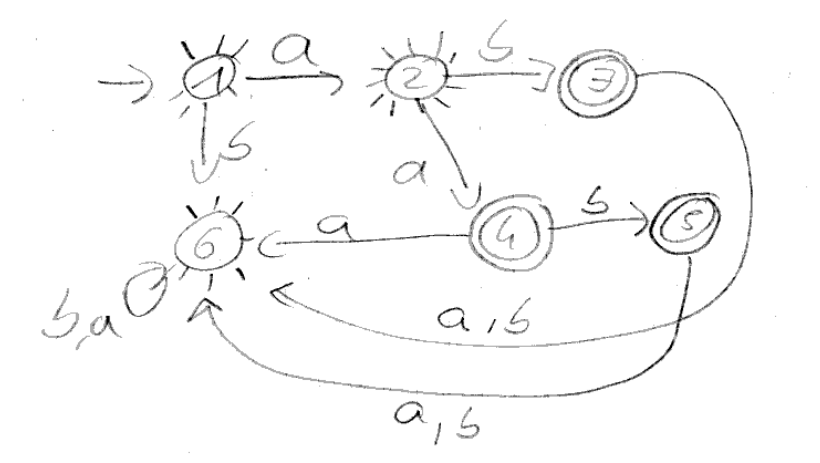
\includegraphics[width=1\linewidth]{Assets/ASK_uebung/u03-01.png}
\end{center}
Idee: Zuerst den Automaten der die aa,ab,aab Sprache akzeptiert aufzeichnen. Dann alle Endzustände (die doppelt umkreisten) zu normalen Zuständen machen und dann die früheren Nicht-Endzustände zu Endzuständen machen (symbolisiert durch die sonnenähnlichen Gebilde um Zustand 1,2,6)

$$L_3 = ((a+b)^*(aa+bb)(a+b)^*(aa+bb)^*(a+b)^*)$$

$$L_4 = (ab)^* + (ba)^*+a+b+\lambda$$


%##########################################
\subsection{Aufgabe 2}
\textit{Zeigen Sie direkt mit dem Pumping-Lemma, dass die Sprache $L=\{a^i b^j \vert i, j\in\mathbb{N}, i > j\}$ nicht regulär ist.}

Behauptung: Die Sprache L ist nicht regulär.
\begin{enumerate}
    \item[0.] Beweis: indirekt. Angenommen L wäre regulär. Nach dem Pumping-Lemma gibt es ein n $\geq$ 1, sodass die folgende Aussage gilt:
          \begin{center}
              Für jedes $x \in L$,  $\mid x \mid \geq n$ gibt es $u,v,w \in\Sigma^*$ mit
              \begin{itemize}
                  \item[i] $x = uvw$
                  \item[ii] $\mid uv \mid\leq n$
                  \item[iii] $\mid v \mid\geq 1$
                  \item[iv] $uv^iw \in L \forall i \geq 0$
              \end{itemize}
          \end{center}
    \item Wir wählen ein Wort $x\in L$. Sei $x = a^nb^j$, wobei n nach Definition der Sprache echt größer $j$ ist.
    \item Nach der Aussage (*) gibt es $u,v,w \in\Sigma^*$, welche die Eigenschaften (i)-(iv) erfüllen.
    \item Sei $x=a^nb^j$ mit $n > j$, wir definieren $j=n-1$.
          Wir wählen $\mid uv \mid < = n$ mit $\mid v\mid\geq k$. Es gilt $v\in\{a\}^+$. Nun sei $i = 0$, damit ist $x=a^{n-k}b^j$, da $\mid v\mid\geq 1$ ist, und da nun $j=n-k$ gilt, ist $n=j$, was allerdings der Bedingung $n>j$ widerspricht. \\
          Wählen wir $\mid v\mid = k$ mit $k\in\mathbb{N}$. so gilt: $uw =a^{(n-k)}b^j$
    \item Dieser Widerspruch von $n = j \neq n > j$ ist ein Widerspruch zu Aussage (iv) des Pumping Lemmas.\\
          Somit ist die Aussage bewiesen, dass die Sprache L nicht regulär sein kann. q.e.d
\end{enumerate}

%##########################################
\subsection{Aufgabe 3}
\textit{Zeigen Sie mit dem Spielschema des Pumping-Lemmas, dass die Sprache $L=\{a^{2^n} | n\in\mathbb{N}\}$ nicht regulär ist.}

\begin{enumerate}
    \item Runde: G wählt eine Zahl $n\geq 1$
    \item Runde: B wählt $x\in L$ mit $\mid x\mid\geq n$. Sei $x = a^{(2^n)}$.
    \item Runde: G wählt $u,v,w$ mit i) $x = u,v,w$ ii) $\mid uv\mid\leq n$ iii) $\mid v\mid\geq 1$
    \item Runde: B wählt $i = 2$ und zeigt, dass $uv^iw \not\in L$ \\
          Sei n beliebig. Wir wählen wie in Runde 2 bereits gesagt $x=a^{2^n}$. Es gilt $x\in L$ und $\mid x\mid\geq n$.\\
          Alle möglichen Stückelungen des Worts sind gemäß der Form: $ u = a^p \quad v = a^q \quad w = a^{2^n}-a^q-a^p$
          mit $p+q \leq n$ und $q\geq 1$.\\
          Wir wählen $i=2$, es gilt $uv^iw = a^{{2^n}+q}$. Es gilt $2^n \geq n \rightarrow p+q < 2^n$ und es gilt weiterhin $0 < q < 2^n$.\\
          Dies bedeutet:$$2^n < 2^n+q < 2^n+2^n = 2*2^n = 2^{n+1}$$
          Hieraus folgt, dass $2^n+q$ keine Zweierpotenz ist, dies wiederum verletzt die Eigenschaften der Sprache und somit ist $uv^iw \notin L$ q.e.d
\end{enumerate}

%##########################################
\subsection{Aufgabe 4}
\textit{Beweisen Sie die folgende verschärfte Version des Pumping-Lemmas: Sei $L\in\sum^*$ eine reguläre Sprache. Dann existiert ein $n>0$, so dass für alle $x\in L$ und alle $x_0,x_1,x_2\in\sum^*$ mit $x=x_0x_1x_2$ und $|x_1|\geq n$ Wörter $u, v, w \in\sum^*$ existieren mit (a) $x_1 = uvw$, (b) $|v| \geq 1$ und
    (c) $x_0 uv^i wx_2\in L$ für alle $i\in\mathbb{N}$.}

Sei $L\subseteq\Sigma^*$ eine reguläre Sprache. Dann exisitiert ein $n>0$, sodass für alle $x\in L$ und alle $x_0,x_1,x_2 \in \Sigma^*$ mit $x = x_0x_1x_2$ und $\mid x_1 \mid \geq n$ Wörter $u,v,w\in \Sigma^*$ existieren mit:
\begin{enumerate}
    \item $x_1$ = uvw
    \item $\mid v \mid \geq 1$ und
    \item $x_0uv^iwx_2 \in L$ für alle $i\in\mathbb{N}$.
\end{enumerate}

Beweis: Sei $n=\mid Z\mid$, wobei Z die Zustände des zugehörigen NFAs $M=(Z,\Sigma,S,\delta,E)$ sind. Ist $x_0x_1x_2 \in L$, so gibt es Zustände $m,n,o\in Z$ mit: $$z_0 \xrightarrow{x_0} m \xrightarrow{x_1} n \xrightarrow{x_2} o \in E$$
Die Transition von m nach n kann in $\mid x_1\mid\geq\mid v\mid +1 \geq n$ Schritten, also durch Begehung von so vielen Zuständen geschehen. Nach der Aussage des Schubkastenprinzips ist dies gleichbedeutend damit, dass zwei der Zustände gleich sein müssen. Nun folgt der Beweis analog dem des einfachen Pumping Lemmas.\\
Es gibt also in $x_1$ Zustände $z_0,z_1,…,z_m$ $\in Z$ mit: $z_0\in S$ (von $x_1$), $z_j \in \delta(z_{j-1},a_j)$ für $1\leq j\leq m$, und $z_m\in E$ (von $x_1$).
Setze $u = a_1 … a_j, v = a_{j+1}…a_k, w=a_{k+1}…a_m$.
Dann gilt:
\begin{itemize}
    \item[i] $x_1 = a_1…a_ja_{j+1}…a_ka_{k+1}…a_m = uvw$ und $x=x_0x_1x_2 = x_0a_1…a_ja_{j+1}…a_ka_{k+1}…a_mx_2 = x_0uvwx_2$
    \item[ii] $\mid uv\mid=\mid a_1…a_k = k \leq n$
    \item[iii] $\mid v\mid = k -(j+1)+1 = k-j > 0$, da ($j < k$)
    \item[iv] Sei $i\geq 0$ beliebig. Es gelten:
          Es führt ein Weg von $z_0\in x_0$ zu dem $z_0^1 \in x_1$ und ein Weg von $z_m^1 \in E \quad von \quad x_1$ nach $z_m \quad von \quad x_2$. Modellieren sozusagen die drei Teilwörter als eigenständige NFAs, bei deren die Überführungen auf die Endzustände der einzelnen NFAs auf die Startzustände des nächsten führen. Betrachten wir nun den NFA zu $x_1$, so folgt nun wie im anderen Beweis auch, dass $uv^iw \in L(x_1)$ ist. Und dies in Kombi mit den weiteren Übergängen $=L$ ist.
\end{itemize}

%##########################################
\subsection{Aufgabe 5}
\textit{Sei $\sum=\{a, b\}$. Wir betrachten die Sprache $L=\{w\in\sum^*\vert\quad |w| \text{ ist gerade und } |w| a \geq 1\}$. Bearbeiten Sie folgende Teilaufgaben:}

\textit{(a) Bestimmen Sie die Myhill-Nerode Äquivalenzklassen von L.}

\textit{(b) Geben Sie den Automaten $M_L$ an}

%##########################################
\subsection{Aufgabe 6}
\textit{Geben Sie einen Algorithmus an, der bei Eingabe eines DFAs M die Größe von $L(M)$ (also $|L(M)|$) berechnet (entweder eine natürliche Zahl $n$ oder $\infty$).}

%##########################################
\subsection{Aufgabe 7}
\textit{Sei $\sum$ ein Alphabet. Zeigen Sie, dass für alle regulären Sprachen $K_1,K_2\subseteq\sum^*$ und ihre Vereinigung $L=K_1\cup K_2$ gilt, dass $Index(R_L)\leq Index(R_{K_1})* Index(R_{K_2})$.}

\newpage
%%%%%%%%%%%%%%%%%%%%%%%%%%%%%%%%%%%%%%%%%%%%%%%%%%%%%%%%%%%%%%%%%%%%%%%%%%%%%%%%%%%%%%%%%%%%%%%%%%%%%%%%%%%%%%%%%%%%
\section{Übung 04}
%##########################################
\subsection{Aufgabe 1}

%##########################################
\subsection{Aufgabe 2}


%##########################################
\subsection{Aufgabe 3}





\newpage
%%%%%%%%%%%%%%%%%%%%%%%%%%%%%%%%%%%%%%%%%%%%%%%%%%%%%%%%%%%%%%%%%%%%%%%%%%%%%%%%%%%%%%%%%%%%%%%%%%%%%%%%%%%%%%%%%%%%
\section{Übung 05}
%##########################################
\subsection{Aufgabe 1}

%##########################################
\subsection{Aufgabe 2}


%##########################################
\subsection{Aufgabe 3}




\newpage
%%%%%%%%%%%%%%%%%%%%%%%%%%%%%%%%%%%%%%%%%%%%%%%%%%%%%%%%%%%%%%%%%%%%%%%%%%%%%%%%%%%%%%%%%%%%%%%%%%%%%%%%%%%%%%%%%%%%
\section{Übung 06}
%##########################################
\subsection{Aufgabe 1}

%##########################################
\subsection{Aufgabe 2}


%##########################################
\subsection{Aufgabe 3}




\newpage
%%%%%%%%%%%%%%%%%%%%%%%%%%%%%%%%%%%%%%%%%%%%%%%%%%%%%%%%%%%%%%%%%%%%%%%%%%%%%%%%%%%%%%%%%%%%%%%%%%%%%%%%%%%%%%%%%%%%
\section{Übung 07}
%##########################################
\subsection{Aufgabe 1}

%##########################################
\subsection{Aufgabe 2}


%##########################################
\subsection{Aufgabe 3}




\newpage
%%%%%%%%%%%%%%%%%%%%%%%%%%%%%%%%%%%%%%%%%%%%%%%%%%%%%%%%%%%%%%%%%%%%%%%%%%%%%%%%%%%%%%%%%%%%%%%%%%%%%%%%%%%%%%%%%%%%
\section{Übung 08}
%##########################################
\subsection{Aufgabe 1}

%##########################################
\subsection{Aufgabe 2}


%##########################################
\subsection{Aufgabe 3}




\newpage
%%%%%%%%%%%%%%%%%%%%%%%%%%%%%%%%%%%%%%%%%%%%%%%%%%%%%%%%%%%%%%%%%%%%%%%%%%%%%%%%%%%%%%%%%%%%%%%%%%%%%%%%%%%%%%%%%%%%
\section{Übung 09}
%##########################################
\subsection{Aufgabe 1}

%##########################################
\subsection{Aufgabe 2}


%##########################################
\subsection{Aufgabe 3}




\newpage
%%%%%%%%%%%%%%%%%%%%%%%%%%%%%%%%%%%%%%%%%%%%%%%%%%%%%%%%%%%%%%%%%%%%%%%%%%%%%%%%%%%%%%%%%%%%%%%%%%%%%%%%%%%%%%%%%%%%
\section{Übung 10}
%##########################################
\subsection{Aufgabe 1}

%##########################################
\subsection{Aufgabe 2}


%##########################################
\subsection{Aufgabe 3}




\newpage
%%%%%%%%%%%%%%%%%%%%%%%%%%%%%%%%%%%%%%%%%%%%%%%%%%%%%%%%%%%%%%%%%%%%%%%%%%%%%%%%%%%%%%%%%%%%%%%%%%%%%%%%%%%%%%%%%%%%
\section{Übung 11}
%##########################################
\subsection{Aufgabe 1}

%##########################################
\subsection{Aufgabe 2}


%##########################################
\subsection{Aufgabe 3}




\newpage
%%%%%%%%%%%%%%%%%%%%%%%%%%%%%%%%%%%%%%%%%%%%%%%%%%%%%%%%%%%%%%%%%%%%%%%%%%%%%%%%%%%%%%%%%%%%%%%%%%%%%%%%%%%%%%%%%%%%
\section{Übung 12}
%##########################################
\subsection{Aufgabe 1}

%##########################################
\subsection{Aufgabe 2}


%##########################################
\subsection{Aufgabe 3}




\newpage
%%%%%%%%%%%%%%%%%%%%%%%%%%%%%%%%%%%%%%%%%%%%%%%%%%%%%%%%%%%%%%%%%%%%%%%%%%%%%%%%%%%%%%%%%%%%%%%%%%%%%%%%%%%%%%%%%%%%
\section{Übung 13}
%##########################################
\subsection{Aufgabe 1}

%##########################################
\subsection{Aufgabe 2}


%##########################################
\subsection{Aufgabe 3}




\newpage
%%%%%%%%%%%%%%%%%%%%%%%%%%%%%%%%%%%%%%%%%%%%%%%%%%%%%%%%%%%%%%%%%%%%%%%%%%%%%%%%%%%%%%%%%%%%%%%%%%%%%%%%%%%%%%%%%%%%
\section{Übung 14}
%##########################################
\subsection{Aufgabe 1}

%##########################################
\subsection{Aufgabe 2}


%##########################################
\subsection{Aufgabe 3}




\newpage
%%%%%%%%%%%%%%%%%%%%%%%%%%%%%%%%%%%%%%%%%%%%%%%%%%%%%%%%%%%%%%%%%%%%%%%%%%%%%%%%%%%%%%%%%%%%%%%%%%%%%%%%%%%%%%%%%%%%
\section{Zusätzliche Aufgaben}

\end{document}